% ============================================================
% 问题4 小节（国赛风格）—— 追加到 001sec.txt 模型建立与问题求解节末尾。
% 数据口径：4-Q4deep 深度求解（tight800，与第三问 A3-codex 同架构）。
% 主结果：末值维持口径（与问题3一致）50.8243 h / 首整分钟 50.8333 h（183000 s）；
%         50°C 设定值口径（并列）51.0875 h / 51.1 h（183960 s）。
% 图片：figures/q4_drying_50°C设定值口径.png、q4_cross.png、
%       q4_convergence.png、q4_scenarios.png、q4_latent.png（复制到论文图片目录后按需改名）。
% ============================================================
\subsection{问题4：考虑尺寸收缩的烘干过程模型}

\subsubsection{问题分析与移动边界变换}

实际烘干中药材因失水而收缩，附件 2 给出烘干过程半径实测序列：半径由
$2.0\ \mathrm{cm}$ 单调收缩至 $1.198\ \mathrm{cm}$（72 h 后维持）。本问在问题 2/3 模型的
基础上引入移动边界 $R(t)$，物性按附录 4 取
\begin{equation}
  \rho(C)=760+90C,\qquad
  c_p(C)=1850+\frac{2150C}{C+1},\qquad
  k(C)=0.12+\frac{0.20C}{C+1},
  \label{eq:props4}
\end{equation}
\begin{equation}
  D(C,T)=4.2\times10^{-4}\exp\Big(-\frac{0.30}{C}\Big)\exp\Big(-\frac{3850}{T}\Big),
  \label{eq:propsD4}
\end{equation}
其中式~\eqref{eq:propsD4} 的 $T$ 为热力学温度。与附录 3 相比，附录 4 扩散前置因子为
其 $1/5.71$、浓度依赖指数更弱（$0.30$ 对 $0.45$），且收缩使有效扩散系数按 $1/R^2$
放大——三者共同决定问题 4 与问题 3 的差异。

引入曲线坐标 $\xi=r/R(t)\in[0,1]$。在\textbf{仿射（均匀）收缩}假设下每个材料点固定在
自身 $\xi$ 上，材料导数即 $\xi$ 坐标下的偏导数，表观对流项恒为零。以随体控制体
$[\xi_1,\xi_2]$ 对水分作衡算：水的内含量为 $2\pi H R^2\int\rho_d C\,\xi d\xi$，跨
$\xi R$ 处的水分总流量为 $-2\pi H\rho_d\,\xi D\,\partial C/\partial\xi$，其中 $\rho_d$ 为
干物质密度；由干物质守恒 $\rho_dR^2=\mathrm{const}$，$R$ 变化引起的项与干物质“压缩项”
严格抵消，$\rho_d$ 完全约去，得
\begin{equation}
  \frac{\partial C}{\partial t}
  =\frac{1}{R^2(t)\,\xi}\frac{\partial}{\partial\xi}\Big(\xi D(C,T)\frac{\partial C}{\partial\xi}\Big),
  \qquad
  \rho(C)c_p(C)\frac{\partial T}{\partial t}
  =\frac{1}{R^2(t)\,\xi}\frac{\partial}{\partial\xi}\Big(\xi k(C)\frac{\partial T}{\partial\xi}\Big),
  \label{eq:mov}
\end{equation}
收缩使内部方程获得 $R^{-2}(t)$ 因子，\textbf{有效扩散系数 $D/R^2(t)$ 随 $R$ 减小而增大}
（最大放大 $(2/1.198)^2=2.79$ 倍），同时改变边界条件、表面面积与固定物理距离的采样
位置——不能表述为“全部影响仅为扩散系数放大”。边界条件为
\begin{equation}
  \xi=0:\ \frac{\partial T}{\partial\xi}=\frac{\partial C}{\partial\xi}=0,\qquad
  \xi=1:\ -\frac{k}{R}\frac{\partial T}{\partial\xi}=h(T_s-T_a),\quad
  -\frac{D}{R}\frac{\partial C}{\partial\xi}=h_m(C_s-C_a),
  \label{eq:movbc}
\end{equation}
初始条件同前两问。$R(t)$ 由附件 2 逐段线性插值给定，超过末观测（259200 s）后维持
$1.198\ \mathrm{cm}$。

\subsubsection{求解方法与烘干时间的确定}

数值离散与问题 3 的 tight800 架构完全一致：表面加密网格
$\xi_{j+1/2}=1-(1-j/N)^2$、$N=800$，界面系数沿相邻状态线性路径三点 Gauss 积分，
真实表面由耦合不动点迭代（半单元与对流串联，残差阈值 $2\times10^{-13}$）解出，表面
通量为 $R\,h(T_s-T_a)$ 与 $R\,h_m(C_s-C_a)$；时间积分用 BDF（`scipy.solve_ivp`，
$\mathrm{rtol}=10^{-11}$、$\mathrm{atol}_T=10^{-12}$、$\mathrm{atol}_C=10^{-13}$，
交错排列块三对角稀疏 Jacobian），前 4 h 每 60 s 数据节点重启，此后以 300 s 为步长上限
连续积分。烘干时间定义为事件时刻
$t^*=\min\{t:\max_r C(r,t)<0.15\ \mathrm{kg/kg}\}$，由终止型事件函数直接根搜索；事件函数取
全场含水率最大值——按 $r^2$ 二次重构的中心值、全部单元值与真实表面值的最大者。由于
全场最大含水率始终位于中心，判据等价于中心判据（已数值印证）。

4 h 后烘房条件的维持方式直接影响长时结果。本文与问题 2/3 保持一致，将附件 1 观测序列
\textbf{按末值维持}（$T_a=50.1650\,^{\circ}\mathrm{C}$、$C_a=0.04986\ \mathrm{kg/kg}$）；
另将“按恒温段设定值 $50.0\,^{\circ}\mathrm{C}$ 维持”作为并列口径给出（恒温段统计
$49.97\pm0.16\,^{\circ}\mathrm{C}$，末点为控制器波动序列的瞬时采样），两种口径相差仅
$0.5\%$，全部结果均落于题面“2–3 天”区间。

\subsubsection{结果与分析}

烘干时间求解结果（末值维持口径）：连续临界时刻为 \textbf{50.8243 h}，按题目 60 s 采样
精度，首次全场严格达标为 \textbf{50.8333 h，即 50 小时 50 分钟（183000 s）}；按恒温段
设定值 $50\,^{\circ}\mathrm{C}$ 维持则为 51.0875 h（首整分钟 51.1 h）。$N=800\to1600$
临界时刻差仅 0.216 s，均匀网格与加密网格相差 0.2 s，数值收敛到秒级。烘干终点半径
$1.2000\ \mathrm{cm}$（附件 2 观测末值 $1.198\ \mathrm{cm}$ 为 72 h 时刻值，非本方案终点）。
表~\ref{tab:C4} 给出题面表 6 格式的水分浓度，图~\ref{fig:drying4} 给出表面与中心的全流程
干燥曲线与半径收缩曲线。

\begin{table}[htbp]
  \centering
  \caption{表 6\quad 药材烘干过程的水分浓度（$\mathrm{kg/kg}$）}
  \label{tab:C4}
  \begin{tabular}{ccccc}
    \hline
    时间/h & \multicolumn{4}{c}{到药材中心的距离/cm} \\
    & 0 & 0.5 & 1.0 & 药材表面 \\
    \hline
    6  & 1.7172 & 1.5357 & 1.0217 & 0.4217 \\
    12 & 0.7343 & 0.6518 & 0.4069 & 0.1667 \\
    18 & 0.4066 & 0.3668 & 0.2388 & 0.0889 \\
    24 & 0.2837 & 0.2599 & 0.1783 & 0.0671 \\
    30 & 0.2253 & 0.2085 & 0.1488 & 0.0593 \\
    36 & 0.1921 & 0.1790 & 0.1312 & 0.0558 \\
    42 & 0.1706 & 0.1598 & 0.1196 & 0.0539 \\
    48 & 0.1556 & 0.1463 & 0.1113 & 0.0529 \\
    50.8333（烘干结束） & 0.1500 & 0.1412 & 0.1081 & 0.0525 \\
    \hline
  \end{tabular}
\end{table}

\begin{figure}[H]
  \centering
  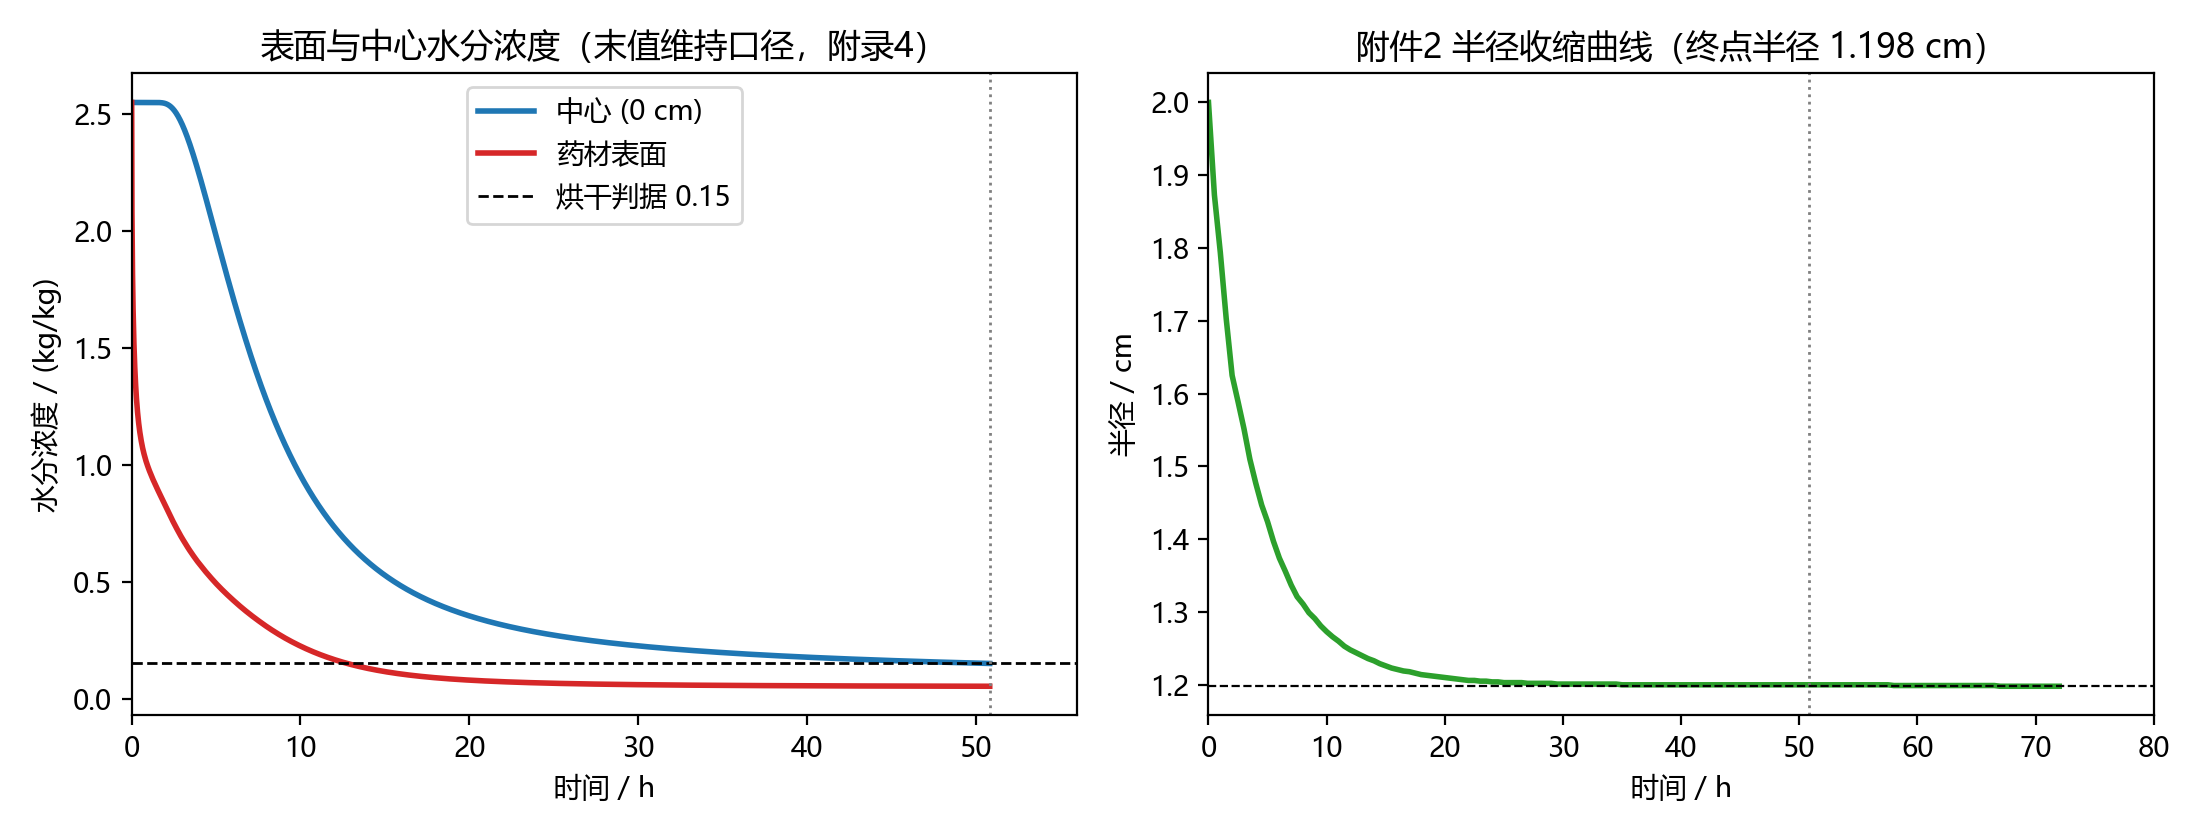
\includegraphics[width=0.9\textwidth]{4-4pic/q4_drying.png}
  \caption{问题 4 全流程干燥曲线（末值维持口径）：表面/中心水分浓度
  与 0.15 判据（左）；附件 2 半径收缩曲线（右，烘干终点半径 1.2000 cm）}
  \label{fig:drying4}
\end{figure}

\textbf{(1) 与问题 3 的交叉：前期更慢、后期更快，约 41.0 h 处交叉。}附录 4 的扩散前置因子
（$4.2\times10^{-4}$）在 $C=2.55$ 时比附录 3（$2.4\times10^{-3}$）小 $5.4$ 倍，故高含水率
阶段问题 4 更慢（6 h 中心 $1.7172$ 对问题 3 的 $1.0156$）；此后收缩使有效系数按
$1/R^2$ 放大（最大 2.79 倍）且附录 4 的浓度依赖 $e^{-0.30/C}$ 弱于附录 3 的
$e^{-0.45/C}$，低含水率阶段反超，中心水分曲线在约 $41.0\ \mathrm{h}$ 处与问题 3 相交
（图~\ref{fig:cross4}）。两个独立模型（不同物性、不同几何处理）给出同量级干时，构成模型族
层面的自洽检验。

\textbf{(2) 收缩的单因素对照。}问题 3 与问题 4 的干时差（57.2 h 对 50.8 h）由物性口径与
几何收缩两项变化共同构成，不能归结为收缩净效应。同为附录 4 物性、固定半径的控制试验
（N=400，末值环境）给出 129.09 h，采用附件 2 收缩半径后为 50.82 h——只改变半径规律的
条件性变化为 $-60.6\%$，该对照不等于与第三组物性模型的比较。表面水分 12 h 即降至
0.1667，此后缓慢逼近烘房平衡值 0.04986。

\textbf{(3) 维持口径的敏感性（最大不确定度）。}4 h 后烘房条件的不同维持口径对烘干时间的
影响为：末值维持（$50.165\,^{\circ}\mathrm{C}$，本文主口径）$50.82$ h、设定值
$50\,^{\circ}\mathrm{C}$ $51.09$ h、末小时均值 $51.10$ h、恒温段均值 $51.14$ h——同一
400 单元网格下最大相对变化 $+0.62\%$（图~\ref{fig:scen4}），小于烘房
$\pm1\,^{\circ}\mathrm{C}$ 引起的 $\mp3.2\%$。两种口径的完整 result4.xlsx 均已交付。

\begin{figure}[H]
  \centering
  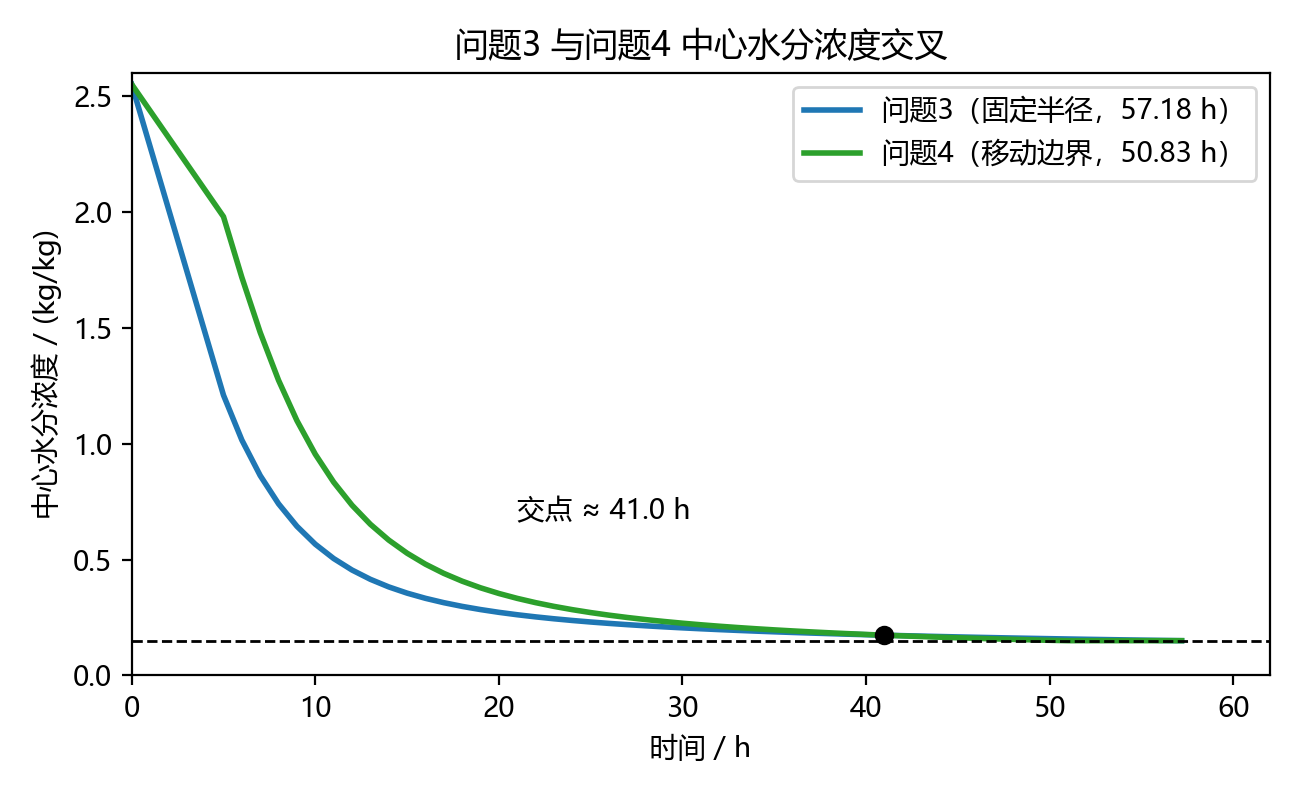
\includegraphics[width=0.62\textwidth]{4-4pic/q4_cross.png}
  \caption{问题 3 与问题 4 中心水分浓度交叉（约 41.0 h 处）}
  \label{fig:cross4}
\end{figure}

\begin{figure}[H]
  \centering
  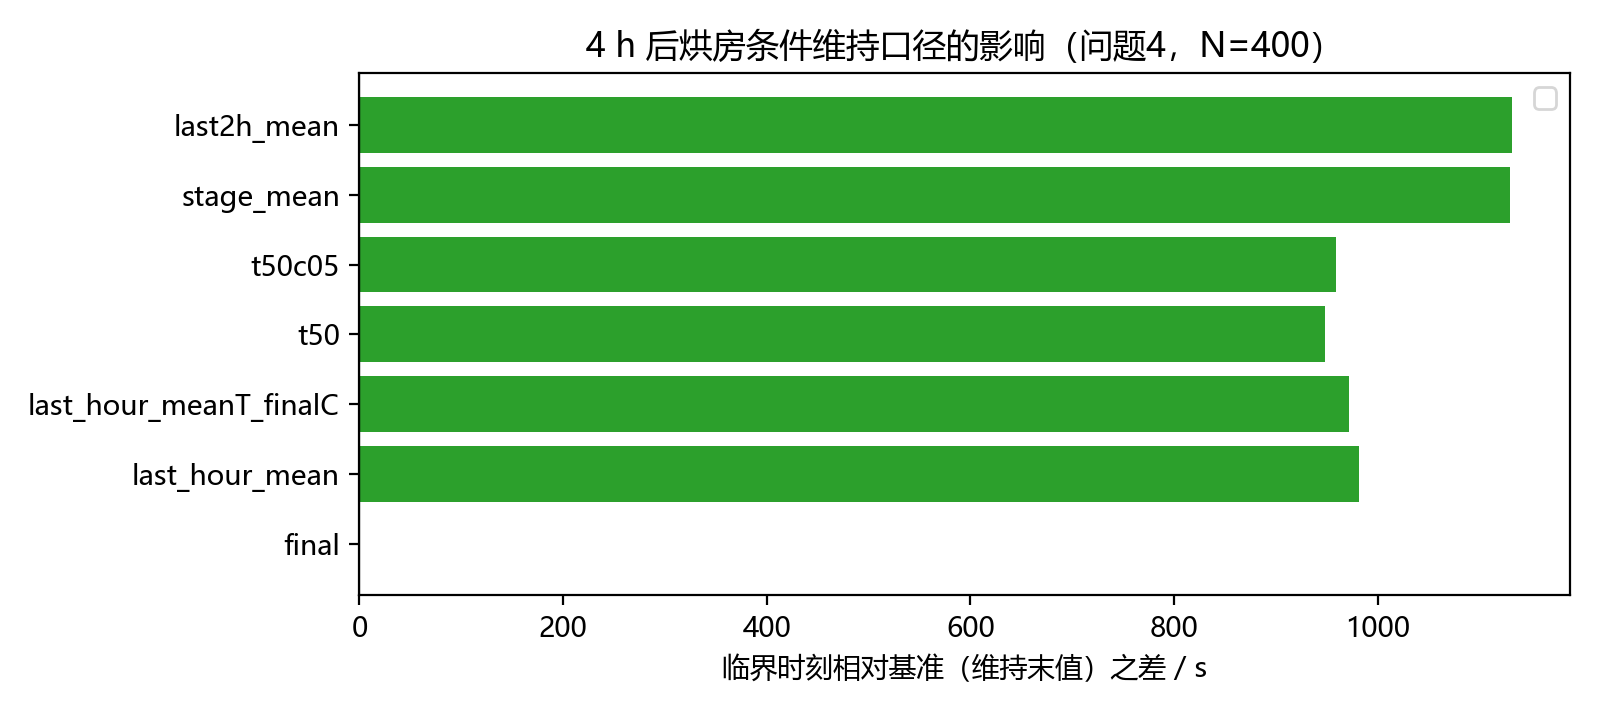
\includegraphics[width=0.85\textwidth]{4-4pic/q4_scenarios.png}
  \caption{4 h 后烘房条件维持口径对问题 4 烘干时间的影响（N=400，相对末值维持基准）}
  \label{fig:scen4}
\end{figure}

\subsubsection{模型检验}

\textbf{(1) 移动边界守恒。}储存量 $M=\sum v_iR^2C_i$ 满足
$\dot M=2R\dot R\sum v_iC_i-R\,j_C$：以三点 Gauss 法积分真实边界通量与体积变化项后，全流程
质量闭合相对残差 $8.90\times10^{-6}$；能量闭合（含变热容链式项与 $2R\dot R$ 项）相对残差
$8.95\times10^{-6}$；离散恒等式
$\sum v_iR^2\dot C_i+q_C=0$、$\sum v_iR^2\rho c_p\dot T_i+q_T=0$ 在全部积分点上达到机器
精度（最大 $4.4\times10^{-16}$）。这些验证说明移动边界变换与通量装配的离散一致性，不替代
未建模物理（端面、吸附等温线等）的讨论。

\textbf{(2) 网格收敛。}$N=400/800/1600$ 表面加密网格的临界时刻为
$182968.1/182967.4/182967.2$ s（$800\to1600$ 差 0.216 s），均匀网格与加密网格相差 0.2 s
（图~\ref{fig:conv4}），临界时刻收敛到秒级；输出列误差小于四位小数阈值
$5\times10^{-5}$，但四位小数的末位仍受舍入分界影响，不作逐位收敛宣称。

\textbf{(3) 与第三问求解器的交叉验证。}同一代码路径切换到附录 3、固定半径后，复现第三问
tight800 的临界时刻 $205810.077$ s（与第三问交付逐位一致），说明移动边界实现未扰动
固定半径路径；全程单元含水率沿径向不增（最大向外增量 $1.3\times10^{-15}$），中心最湿
判据成立。

\begin{figure}[H]
  \centering
  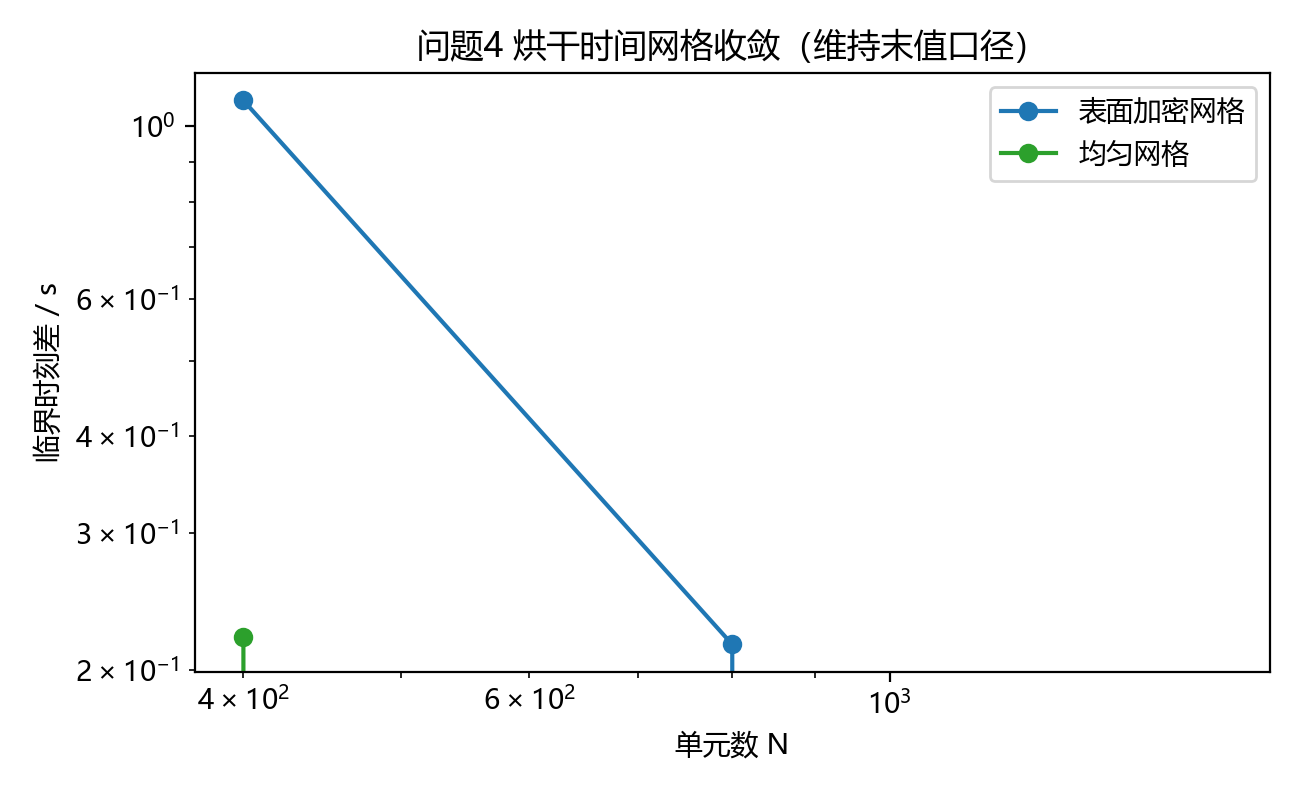
\includegraphics[width=0.62\textwidth]{4-4pic/q4_convergence.png}
  \caption{问题 4 烘干时间的网格收敛（表面加密与均匀网格，末值维持口径）}
  \label{fig:conv4}
\end{figure}

\textbf{(4) 潜热项对照。}在表面能量边界补入蒸发潜热流 $L_v\rho_d h_m(C_s-C_a)$（换算密度取
干物质密度锚定值 $\rho_d=\rho(C_0)/(1+C_0)=278.7\ \mathrm{kg/m^3}$，$L_v=2383\ \mathrm{kJ/kg}$）
后，烘干时间为 56.16 h（$+10.5\%$，末值口径），体积型汇为 58.25 h（$+14.6\%$）；单位
系数试验仅为人工敏感性分析，不是物理标定值。目前没有证据表明潜热已被题面经验参数吸收，
不含潜热是基准简化假设、含潜热是明确密度换算后的替代模型，二者并列呈现；不能仅凭某组
数值接近参考值来选择模型。潜热对照仅作为模型讨论，不作为正式答案。

综上，考虑尺寸收缩后药材烘干所需时间为 \textbf{50.8333 h（2.12 天）}，烘干终点半径
$1.2000\ \mathrm{cm}$（72 h 观测末值 $1.198\ \mathrm{cm}$ 非本方案终点半径）；与问题 3 的
差异为物性口径与几何收缩两项变化之和（见上文单因素对照）。完整结果按模板输出至
result4.xlsx（60 s $\times$ 0.1 cm，列 0–1.1 cm + 药材表面，3050 行，4 位小数），末行
中心显示 0.1500 为四位小数舍入所致（未舍入值 $0.14999\ldots$，严格达标按未舍入值判定）。
